\documentclass[10pt, a4paper]{beamer}

\usepackage{color}
\usepackage{graphicx}



\usepackage{xcolor,colortbl}
\usepackage[export]{adjustbox}
\definecolor{Gray}{gray}{0.85}
\definecolor{LightCyan}{rgb}{0.88,1,1}


\usetheme{Berkeley}
\usecolortheme{crane}

\begin{document}
	\setbeamertemplate{sidebar left}{}	
	\title{Progress Presentation-I}
	\subtitle{e-Yantra Summer Intership-2015 \\ Marker based localisation }
	\author{\textbf{Niharika Jayanthi}\\ \textbf{Dheeraj Kamath}\\
	\textcolor{black}{Mentor: \textbf{Sanam Shakya}}}
	\institute{IIT Bombay}
	\date{\today}
	%\addtobeamertemplate{sidebar left}{}{\includegraphics[scale = 0.3]{logowithtext.png}}
	\frame{\titlepage}

\setbeamertemplate{sidebar left}[sidebar theme]
\section{Overview of Project}
\begin{frame}{Overview of Project}

	\begin{itemize}
		\pause
		\item  Marker based localisation
		\pause
		\item Objective: To develop modules for Image Processing and robot localisation using markers
		\pause
		\item Deliverables:\begin{enumerate}
			\item Develop modules for: \\
			      1. Morphological operation \\
			      2. Image filtering operation \\
			      3. Lines and contour detection \\
			      4. Shape detection
			\pause
			\item 	Robot which is capable of recognizing the markers and localize in the indoor environment. For testing, robot will be placed in the predefined environment with markers. Then robot should give the (x, y) coordinate in the room.
			\pause
			\item 	Robot which is capable of moving between two random way points in the room with markers.
		 	
		                     \end{enumerate}
	\end{itemize}
\end{frame}

\section{Overview of Task}
\begin{frame}{Overview of Task}
	\centering
	\begin{tabular}{ c  p{6cm}  c }
	
		\\
			\rowcolor{LightCyan}
		Task no & \centering Tasks & Deadlines  \\
		\hline
		\\
		\rowcolor{LightCyan}
		1 & \small{Installation of required softwares on raspberry pi and documentation } & 2 days\\
		\hline
		\\
		\rowcolor{LightCyan}
		2 & Develop modules for morphological operation with documentation & 3 Days\\
		\hline
		\\
		\rowcolor{LightCyan}
		3 & Develop modules for image filtering operation  with documentation & 2 Days\\
		\hline
		\\
		\rowcolor{LightCyan}
		4 & Develop modules for extracting lines and contours with documentation & 3 Days \\
		\hline \\
		
		
     \end{tabular}
\end{frame}

\section{Overview of Task}
\begin{frame}{Overview of Task}
	\framesubtitle{cont...}
	\centering
	\begin{tabular}{ c  p{6cm}  c }
		\\
		\rowcolor{LightCyan}
		Task no & \centering Tasks & Deadlines  \\
		\hline
		\\
		\rowcolor{LightCyan}
		5 & Creation of various shape detectors for shape detection with documentation  & 3 Days \\
		\hline
		\\
		\rowcolor{LightCyan}
		6 & Design a marker and develop the marker detection and recognition algorithm & 3 Days  \\
		\hline
		\\
		\rowcolor{LightCyan}
		7 & \small{Camera calibration and pose estimation and recognition algorithm} & 2 days\\
		\hline
		\\
		\rowcolor{LightCyan}
		8 & Mapping the robot position from the data obtained from the marker& 5 Days \\
		\hline
		\\
		\rowcolor{LightCyan}
		9 & Create path from source to destination waypoints with the help of visual markers & 6 Days \\
		
		\hline
		
	\end{tabular}
\end{frame}

\section{Task Accomplished}
\begin{frame}{Task 1}{Setting up of Raspberry Pi}
	\pause
	\begin{itemize}
		\item \textbf{Setup of the Raspberry Pi}\\
		\pause
		\begin{block}{Raspberry Pi is a small,low-cost, powerful credit card sized computer that was developed to promote education among adults and children alike.}
		\end{block}
		\pause
         \centering
		\begin{figure}[!htb]
			\begin{minipage}{0.5\textwidth}
				\centering
		    	\includegraphics[width=0.5\linewidth,height = 0.4\textheight,left]{C:/Users/KUMAR/eYSIP_2015_Marker_based_Robot_Localisation.wiki/images/ras.jpg}
		    	
		    \label{fig:sfig2}
		    \end{minipage}
		    \centering
		    \caption{Raspberry Pi}
		    \label{fig:fig}
		
	\end{figure}	
		
		
	 \end{itemize}
	 
\end{frame}


\begin{frame}{Steps Involved}
	\begin{itemize}
	  	\item Download Raspbian and win32DiskManager softwares.
	  	\item  Insert your sd card.Run win32DiskImager and choose the Raspbian image and select the drive corresponding to your sd card. 
	  	\item Insert it into the sd card slot of the Raspberry Pi.
	  	\item .Use HDMI cable to connect the board to the monitor/tv.
	  	Power on the board and the monitor. You will notice a set of code running on the monitor.
	  	\item  It opens a software configuration tool.
	    
	\end{itemize}
\end{frame}

\begin{frame}{Steps Involved}
	
		\begin{minipage}{0.5\textwidth}
			\centering
			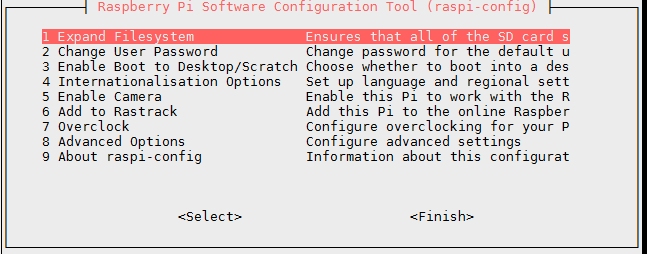
\includegraphics[width=1.8\linewidth,height = 0.5\textheight,left]{C:/Users/KUMAR/eYSIP_2015_Marker_based_Robot_Localisation.wiki/images/Raspi-config.png}
			\label{fig:sfig2}
		\end{minipage}
	
\end{frame}

\begin{frame}{Task 2}{Thresholding}
	\begin{itemize}
		\item Simplest method of image segmentation
		\item Can be used to create binary images from grayscale images
		\item Pixels compared with threshold value
	\end{itemize}
	\begin{minipage}{0.5\textwidth}
		\centering
		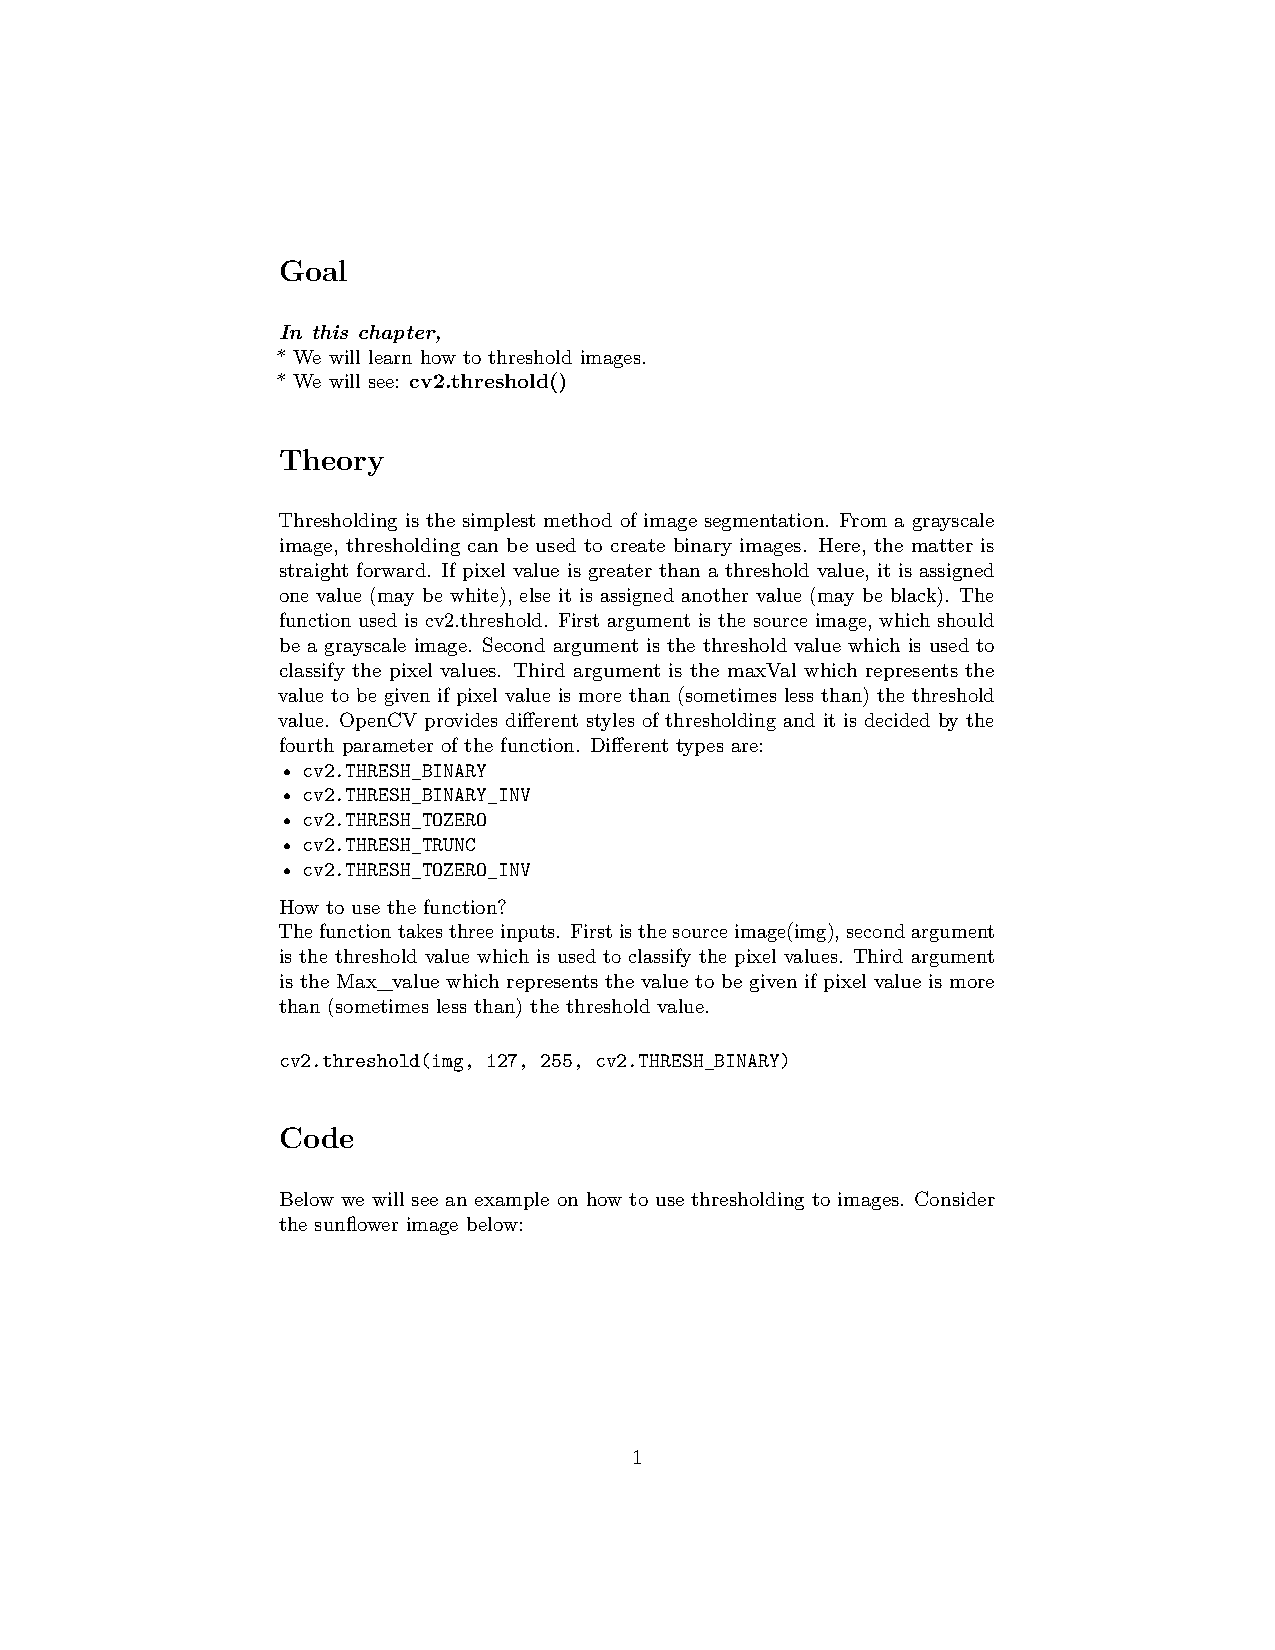
\includegraphics[width=1.5\linewidth,height = 0.7\textheight,left]{C:/Users/KUMAR/eYSIP_2015_Marker_based_Robot_Localisation.wiki/images/Thresholding.png}
		\label{fig:sfig3}
		
		
	\end{minipage}	
\end{frame}		


\begin{frame}{Task 2}{Morphological Operations}
	\
	\begin{itemize}
		\item[$\bullet$] \textbf{Erosion}
		\\Erodes the boundaries of an object image
		\item[$\bullet$] \textbf{Dilation}
		\\Increases the size of boundary of image
		\item[$\bullet$] \textbf{Opening}
		\\Erosion followed by dilation
		\item[$\bullet$] \textbf{Closing}
		\\Dilation followed by erosion	
	\end{itemize}
\end{frame}
\begin{frame}{Task 2}{Morphological Operations}
	
	\begin{minipage}{0.5\textwidth}
		\centering
		\includegraphics[width=1.5\linewidth,height = 0.7\textheight,left]{C:/Users/KUMAR/eYSIP_2015_Marker_based_Robot_Localisation.wiki/images/morph.png}
		
		
	\end{minipage}		
	
\end{frame}	




\begin{frame}{Task 2}{Distance Transform}
	\
	Distance transform is used to modify a image to display its skeleton.\\ \ \\
	\textbf{How is the image modified?}\\
	The closer a pixel is to the boundary of the object image, the darker it is (i.e. it has a lower value).\\
	In this way, the center (or the skeleton) of the image is highlighted.
	\begin{minipage}{0.5\textwidth}
		\centering
		\includegraphics[width=1.5\linewidth,height = 0.7\textheight,left]{C:/Users/KUMAR/eYSIP_2015_Marker_based_Robot_Localisation.wiki/images/tiger_DT.png}
		\label{fig:sfig4}
		
		
	\end{minipage}		
	
\end{frame}



\begin{frame}{Task 2}{Watershed Segementation}
	Watershed is an algorithm in image processing used for isolating objects in the image from the background.
	\begin{minipage}{0.5\textwidth}
		\centering
		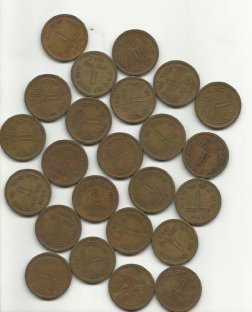
\includegraphics[width=1\linewidth,height = 0.7\textheight,left]{C:/Users/KUMAR/eYSIP_2015_Marker_based_Robot_Localisation.wiki/images/water_coins.jpg}
		\label{fig:sfig4}
		
		
	\end{minipage}		
	
\end{frame}		
\begin{frame}{Task 2}{Watershed Segementation}
Step 1: 

	\begin{minipage}{0.5\textwidth}
		\centering
		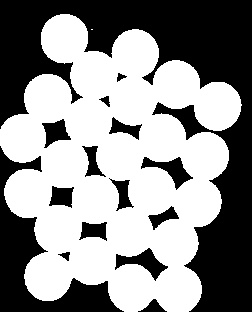
\includegraphics[width=1\linewidth,height = 0.7\textheight,left]{C:/Users/KUMAR/eYSIP_2015_Marker_based_Robot_Localisation.wiki/images/otsuthresh.jpg}
		\label{fig:sfig4}
		
		
	\end{minipage}		
	
\end{frame}		
		

\begin{frame}{Task 2}{Watershed Segementation}
	Step 2: 
	
	\begin{minipage}{0.5\textwidth}
		\centering
		\includegraphics[width=1\linewidth,height = 0.7\textheight,left]{C:/Users/KUMAR/eYSIP_2015_Marker_based_Robot_Localisation.wiki/images/Sure_fg.jpg}
		
		
		
	\end{minipage}		
	
\end{frame}		
\begin{frame}{Task 2}{Watershed Segementation}
	Step 3: 
	
	\begin{minipage}{0.5\textwidth}
		\centering
		\includegraphics[width=1\linewidth,height = 0.7\textheight,left]{C:/Users/KUMAR/eYSIP_2015_Marker_based_Robot_Localisation.wiki/images/Sure_bg.jpg}
		\label{fig:sfig4}
		
		
	\end{minipage}		
	
\end{frame}		
\begin{frame}{Task 2}{Watershed Segementation}
	Step 4: 
	
	\begin{minipage}{0.5\textwidth}
		\centering
		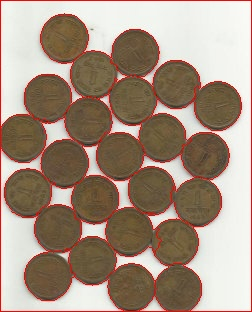
\includegraphics[width=1\linewidth,height = 0.7\textheight,left]{C:/Users/KUMAR/eYSIP_2015_Marker_based_Robot_Localisation.wiki/images/img.jpg}
		\label{fig:sfig4}
		
		
	\end{minipage}		
	
\end{frame}		

\begin{frame}{Task 3}{Gradients}
	\begin{block} {Three commonly used methods to find gradients: }\end{block}
	\begin{itemize}
		\item Scharr
		\item Sobel
		\item Laplacian
		
	\end{itemize}	
\end{frame}	
\begin{frame}{Task 3}{Gradients}

	\begin{minipage}{0.5\textwidth}
		\centering
		\includegraphics[width=1.5\linewidth,height = 0.7\textheight,left]{C:/Users/KUMAR/eYSIP_2015_Marker_based_Robot_Localisation.wiki/images/grad.png}

		
		
	\end{minipage}		
	
	
	
\end{frame}	

\begin{frame}{Task 3}{Blur}
	Types of blurring techniques:\\
		\begin{minipage}{0.5\textwidth}
			\centering
			\includegraphics[width=1.5\linewidth,height = 0.7\textheight,left]{C:/Users/KUMAR/eYSIP_2015_Marker_based_Robot_Localisation.wiki/images/mona.png}
			\label{fig:sfig4}
			
			
		\end{minipage}		
	

		
\end{frame}			

\begin{frame}{Task 3}{Line Detection}

	\begin{itemize}
		\item \textbf{Canny Edge Detection}\\
		As the name suggests, this algorithm is used to detect the edges in an object image.
		
		
	\end{itemize}
	\begin{minipage}{0.5\textwidth}
		\centering
		\includegraphics[width=1\linewidth,height = 0.7\textheight,left]{C:/Users/KUMAR/eYSIP_2015_Marker_based_Robot_Localisation.wiki/images/cartoon_ab.jpg}
		\label{fig:sfig4}
		
		
	\end{minipage}	
		
\end{frame}	
\begin{frame}{Task 3}{Line Detection}
	And the answer is ...\\
	\begin{minipage}{0.5\textwidth}
		\centering
		\includegraphics[width=1\linewidth,height = 0.7\textheight,left]{C:/Users/KUMAR/eYSIP_2015_Marker_based_Robot_Localisation.wiki/images/ab2.jpg}
		\label{fig:sfig4}
		
		
	\end{minipage}	
	
	
\end{frame}	
\begin{frame}{Task 3}{Line Transform}
	\textbf{Hough Line Transform}\\
	\begin{itemize}
		\item Feature extraction technique
		\item Purpose: Find imperfect instances of objects
		\begin{block}{How is the line detected?}\end{block}
		\item Intersections between curves
    \end{itemize}	
    \begin{minipage}{0.5\textwidth}
    	\centering
    	\includegraphics[width=1.7\linewidth,height = 0.7\textheight,left]{C:/Users/KUMAR/eYSIP_2015_Marker_based_Robot_Localisation.wiki/images/Hough.png}
    	\label{fig:sfig4}
    	
    	
    \end{minipage}
\end{frame}	




\begin{frame}{Task 4}{Shape Detection}
 	\begin{block}{Detection and identification of various shapes by:} \end{block}
	\begin{itemize}
		\item Uses Hu moments to compare two objects
		\item Identifying the shape based on number of vertices
	\end{itemize}
	\begin{minipage}{0.5\textwidth}
		\centering
		\includegraphics[width=1.5\linewidth,height = 0.7\textheight,left]{C:/Users/KUMAR/eYSIP_2015_Marker_based_Robot_Localisation.wiki/images/Shape.png}
		\label{fig:sfig4}
		
		
	\end{minipage}
	
	
\end{frame}	

\section{Challenges Faced}
\begin{frame}{Challenges Faced}
	\begin{itemize}
		
		\item[$\bullet$] Configuring wifi settings in Raspberry Pi
		\item[$\bullet$] Installation of opencv in MAC OSX
		\item[$\bullet$] Difference in bitness of Python and module to be installed(modules like matplotlib and numpy)
		\item[$\bullet$] Counting of overlapping object using watershed segmentation
		\item[$\bullet$] Lane detection with extraneous objects on the road
	\end{itemize}
\end{frame}

\section{Future Plans}
\begin{frame}{Future Plans}
	\begin{block}{By the next project presentation, we aim to accomplish the following:}\end{block}
	\begin{itemize}
		\item Develop marker detection and recognition algorithm
		\item Develop pose estimation algorithm by calibrating the camera
		\item Map the robot's position by the data obtained from the marker
		
	\end{itemize}
\end{frame}


\section{Thank You}
\begin{frame}{Thank You}
	\centering \Large{THANK YOU !!!}\\
    \small Any questions?
\end{frame}
\end{document}
